%TODO: CORREGIR COMANDOS PARA QUE SE VEAN CON VERB
%TODO: INTENTAR QUITAR LA MORRAYA QUE NO SIRVA
%TODO: INTENTAR NO REPETIR TANTAS COSAS EN EL EJERCICIO 3
%TODO: REVISAR DOCUMENTO PARA FALLOS ORTOGRAFICOS/GRAMATICALES
\documentclass{article}
\usepackage[utf8]{inputenc}
\usepackage[spanish]{babel}
\usepackage{graphicx, graphics, float, hyperref}
\usepackage{listings, subcaption}
\usepackage[a4paper, total={6in, 10in}]{geometry}

\title{SSO Práctica 4 Sesión 1}
\author{Andrés Merlo Trujillo}
\date{}
\hypersetup{
    colorlinks=true,
    linkcolor=black,
}

\begin{document}

\maketitle

\tableofcontents

\newpage
%\addcontentsline{toc}{section}{Ejercicio 1}
%\section*{Ejercicio 1}
%\begin{figure}[H]
%    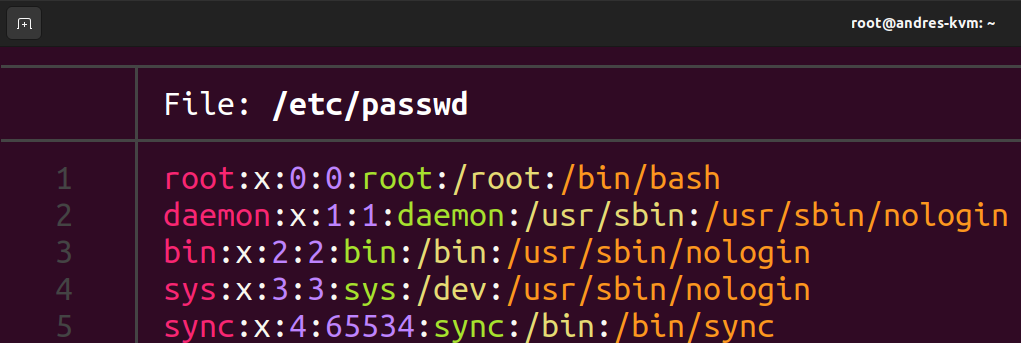
\includegraphics[width=\textwidth]{imagenes/passwdfile.png}
%    \caption{Ejemplo de entradas en el archivo.}
%\end{figure}

\addcontentsline{toc}{section}{Ejercicio 1}
\section*{Ejercicio 1}

Debido a que le pendrive que tengo es muy lento (usa USB 2.0), voy a crear una particion de 1 GB con el sistema de archivos ext4.

Y ahora a modo de realismo, voy a copiar las imagenes usadas durante estas practicas y un archivo dentro de la carpeta ``mis trabajos'' denominado ``amenaza.txt'' con una frase que amenace.

%Foto de la carpeta con archivos y del archivo amenaza

A continuacion desmonto el disco para suponer que he recibido el pendrive asi y para que no pueda realizarle mas modificaciones.

Ahora voy a seguir los pasos indicados en el guion de practicas, por tanto, lo primero que hay que hacer es obtener la estructura interna de particiones con la orden \verb|fdisk -l /dev/sdX > fdisk.disco1| siendo la X la letra asignada al disco, en mi caso es a. (se puede comprobar con la orden \verb|fdisk -l| o \verb|lsblk|).

%foto de la salida del comando

Lo siguiente que hay que hacer es crear una imagen forense del disco para evitar invalidar el contenido del pendrive y trabajar de forma segura sobre una copia. Esto se realiza mediante la orden \verb|dd if=/dev/sda1 of=imagen.disco1 bs=512|.

%salida de dd


\end{document}
